\documentclass{article}

\ExplSyntaxOn
\cs_set_eq:NN
\etex_iffontchar:D
\tex_iffontchar:D
\cs_undefine:N \c_one
\int_const:Nn \c_one{1}
\ExplSyntaxOff
\usepackage{amsmath,tikz, amsthm, amssymb}
\usetikzlibrary{matrix}
\usepackage{physics}
\usepackage{xepersian}
\settextfont{Yas}
\setdigitfont{Yas}
\theoremstyle{remark}		%for the examples are in italics, so we need this fix for it to be normal
\newtheorem{example}{مثال}		% withh * it would not have any counters whatsoever
\newtheorem*{varsol}{حل}
\title{برازش منحنی به کمک معیار کم‌ترین مربعات و تجزیه $SVD$}

\begin{document}
	\maketitle

%	\{حل مساله کمترین مربعات با تجزیه ی $SVD$}
	مساله ی کم ترین مربعات زیر را در نظر بگیرید: 
	
	\begin{flushleft}
		$min\norm {b-AX}_2 \ \ \ \  X \in \mathbb{R}^n$
	\end{flushleft}
فرض کنیم  تجزیه ی مقدار منفرد ماتریس $A$ به صورت زیر باشد:
\begin{flushleft}
	$A=USV^\top$
\end{flushleft}
خواهیم داشت: 
\begin{flushleft}
	$\norm{b-AX}_2 = \norm{b-USV^\top X}_2 =\norm{U^\top b - SV^\top X}_2$
\end{flushleft}
حال قرار می دهیم: 
\begin{center}
	$C=U^\top b , \ Z = V^\top X$
\end{center}
\begin{equation*}
	 SV^\top X = SZ = 
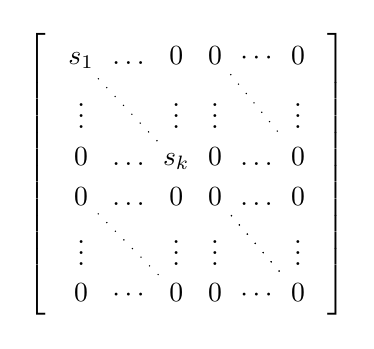
\begin{tikzpicture}[baseline=(current bounding box.center)]
	\matrix (m) [matrix of math nodes,nodes in empty cells,right delimiter={]},left delimiter={[} ]{
		s_1  & \dots & 0  &  0 & \cdots & 0  \\
		\vdots & & \vdots&  \vdots& & \vdots \\
		0 &\dots &s_k &0 & \dots & 0 \\
		0 &\dots & 0& 0 & \dots& 0   \\
		\vdots	& & \vdots & \vdots & &  \vdots \\
		0 & \cdots & 0& 0 & \cdots & 0 \\
	} ;
	\draw[loosely dotted] (m-4-1)-- (m-6-3);
	\draw[loosely dotted] (m-4-4)-- (m-6-6);
	\draw[loosely dotted] (m-1-4)-- (m-3-6);
	\draw[loosely dotted] (m-1-1)-- (m-3-3);
	\draw[loosely dotted] (m-4-4)-- (m-6-6);
\end{tikzpicture}
\begin{bmatrix}
	z_1 \\
	z_2 \\ 
	\vdots \\
	z_n
\end{bmatrix} = 
\begin{bmatrix}
	s_1 z_1 \\ 
	\vdots \\
	s_k z_k \\
	0 \\
	\vdots \\
	0
\end{bmatrix}
\end{equation*}
\begin{flushleft}
	 $\implies \norm{b-AX}_2 = \norm{[c_1 - s_1 z_1, \ c_2 - s_2 z_2, \ \cdots , c_k - s_k z_k , c_{k+1},  \cdots , c_m]}_2$
\end{flushleft}
\begin{flushleft}
	$= (\sum\limits_{i=1}^{k} (c_i-s_iz_i)^2 + \sum\limits_{i=k+1}^{m}c^2_i)^{1/2}$
\end{flushleft}
و این عبارت زمانی می نیمم می شود که:
\begin{flushleft}
	\[
	z_i = 
	\begin{cases}
		\frac{c_i}{s_i}, & i\leq i \leq k \\
		\text{دلخواه}, & k < i \leq n
	\end{cases}
	\]
\end{flushleft}
با مشخص شدن بردار Z ، با توجه به تساوی $Z=V^\top X$ ، بردار مجهول $X$ از رابطه ی $X=VZ$ محاسبه می شود. \\
\begin{example}
با استفاده از تجزیه ی  $SVD$ ، چند جمله ای درجه ی دو را طوری بیابید که با معیار کم ترین مربعات بهترین تقریب داده های زیر باشد.\\
\begin{flushleft}
\begin{tabular}{l | l}
	$y_i$ & $x_i$ \\
	\hline
	1 & 0 \\
	$1.2840$ & $0.25$  \\
	$1.6487$ & $0.5$   \\
	$2.1170$ & $0.75$  \\
	$2.7183$ & $1.00$  
\end{tabular}
\end{flushleft}

\end{example}
\begin{varsol}
	چند جمله ای درجه ی دو $p_2$ را به صورت زیر در نظر می گیریم.
	\[
	p_2(x) = a_0  + a_1 x + a_2 x^2
	\]
	هدف یافتن ضرایب $a_0$ $a_1$ و $a_2$ می باشد. اگر داده های $(x_i, y_i)$ در چند جمله ای فوق صدق می کرد به ازای $i=1,\cdots ,5$ ، تساوی $p_2(x_i) = y_i $ برقرار می بود، یعنی: \\
	\begin{equation*}
	\begin{tabular}{c c }
		 $a_0 +a_1x_1 + a_2x_1^2 = y_1$ & $i=1:$ \\
		 $a_0 + a_1x_2 + a_2x_2^2 = y_2$  & $i= 2:$ \\
		 $a_0 + a_1x_3 + a_2x_3^2 = y_3$  & $i= 3:$ \\
		 $a_0 + a_1x_4 + a_2x_4^2 = y_4$  & $i= 4:$ \\
		 $a_0 + a_1x_5 + a_2x_5^2 = y_5$  & $i= 5:$ 
	\end{tabular} \implies 
%\overbrace{hello}
\begin{bmatrix}
	1 & x_1 & x_1^2 \\
	1 & x_2 & x_2^2 \\
	1 & x_3 & x_3^2 \\
	1 & x_4 & x_4^2 \\
	1 & x_5 & x_5^2
\end{bmatrix}
\begin{bmatrix}
	a_0\\
	a_1\\
	a_2
\end{bmatrix} = 
\begin{bmatrix}
	y_1 \\
	y_2 \\
	y_3 \\
	y_4 \\ 
	y_5
\end{bmatrix}
	\end{equation*}
و با جای گذاری $x_i$ و $y_i$ ها: \\
\begin{equation}
	\stackrel{\mbox{$A$}}{%
	\begin{bmatrix}
		1 & 0 & 0 \\
		1 & $0.25$ & $0.0625$ \\
		1 & $0.5$ & $0.25$ \\
		1 & $0.75$ & $0.5625$ \\
		1 & 1 & 1
	\end{bmatrix}
}
	\stackrel{\mbox{$X$}}{%
	\begin{bmatrix}
		a_0 \\
		a_1 \\
		a_2 
	\end{bmatrix}
} = 
	\stackrel{\mbox{$b$}}{%
	\begin{bmatrix}
		1 \\
		$1.2840$ \\
		$1.6487$ \\
		$2.1170$ \\
		$2.7183$
	\end{bmatrix}
}
\end{equation}
اما این دستگاه جواب ندارد، لذا با معیار کم ترین مربعات، می خواهیم بردار $
\begin{bmatrix}
	a_0 \\ 
	a_1 \\ 
	a_2
\end{bmatrix}$
را طوری بیابیم که $\norm{b-AX}_2$ را می نیمم کند. تجزی ی $SVD$ ماتریس A به صورت زیر به دست می آید: \\
\[
A = USV^\top
\]
\[
U = 
\begin{bmatrix}
	$-0.29$ & $-0.63$ & $0.63$ & $-0.014$ & $-0.3378$ \\ 
	$-0.34$ & $-0.45$ & $-0.21$ & $0.255$ & $0.75$ \\ 
	$-0.41$ & $-0.19$ & $0.52$ & $-0.68$ & $-0.22$ \\ 
	$-0.50$ & $-0.14$ & $0.31$ & $-0.65$ & $-0.45$ \\ 
	$-0.60$ & $0.57$ & $0.43$ & $-0.21$ & $-0.2678$ 
\end{bmatrix}
\]
\[
S = 
\begin{bmatrix}
	$2.71$ & 0 & 0 \\
	0 & $0.9371$ & 0 \\
	0 & 0 & $0.1627$ \\
	0 & 0 & 0 \\
	0 & 0 & 0
\end{bmatrix} , \  V^\top = 
\begin{bmatrix}
	$-0.79$ & $-0.47$ & $-0.37$ \\  
	$-0.59$ & $0.51$ & $0.62$ \\  
	$0.1027$ & $0.71$ & $0.68$ 
\end{bmatrix}
\]
\[
C = U^\top b =  U^\top 
\begin{bmatrix}
	y_1 \\
	y_2 \\
	y_3 \\
	y_4 \\
	y_5
\end{bmatrix} = 
\begin{bmatrix}
	$-4.1372$ \\
	$0.3473$ \\ 
	$0.0099$ \\
	$-0.0059$ \\ 
	$0.0155$
\end{bmatrix}
\]
\\
\[
z_1 = \frac{c_1}{s_1}  = -1.526 , \ z_2 = \frac{c_2}{s_2}  = 0.3706 , \ z_3 = \frac{c_3}{s_3}  = 0.0609
\]
\\
\[
X = 
\begin{bmatrix}
	a_0 \\
	a_1 \\
	a_2
\end{bmatrix}, \ VZ =  
\begin{bmatrix}
	$1.005$ \\
	$0.8642$ \\
	$0.8437$
\end{bmatrix}
\]
\[
P_2(x)  =  1.005 + 0.8642x + 0.8437x^2
\]
	\end{varsol}
\end{document}